\documentclass[aspectratio=169,t,11pt,table]{beamer}
% xcolor and define colors -------------------------
\usepackage{xcolor}

% https://www.viget.com/articles/color-contrast/
\definecolor{purple}{HTML}{5601A4}
\definecolor{navy}{HTML}{0D3D56}
\definecolor{ruby}{HTML}{9a2515}
\definecolor{alice}{HTML}{107895}
\definecolor{daisy}{HTML}{EBC944}
\definecolor{coral}{HTML}{F26D21}
\definecolor{kelly}{HTML}{829356}
\definecolor{cranberry}{HTML}{E64173}
\definecolor{jet}{HTML}{131516}
\definecolor{asher}{HTML}{555F61}
\definecolor{slate}{HTML}{314F4F}

% Mixtape Sessions
\definecolor{picton-blue}{HTML}{00b7ff}
\definecolor{violet-red}{HTML}{ff3881}
\definecolor{sun}{HTML}{ffaf18}
\definecolor{electric-violet}{HTML}{871EFF}

\newcommand\pictonBlue[1]{{\color{picton-blue}#1}}
\newcommand\sun[1]{{\color{sun}#1}}
\newcommand\electricViolet[1]{{\color{electric-violet}#1}}
\newcommand\violetRed[1]{{\color{violet-red}#1}}

\newcommand\bgPictonBlue[1]{{\colorbox{picton-blue!20!white}{#1}}}
\newcommand\bgSun[1]{{\colorbox{sun!20!white}{#1}}}
\newcommand\bgElectricViolet[1]{{\colorbox{electric-violet!20!white}{#1}}}
\newcommand\bgVioletRed[1]{{\colorbox{violet-red!20!white}{#1}}}

\def\code#1{\texttt{#1}}

% Main theme colors
\definecolor{accent}{HTML}{00b7ff}
\definecolor{accent2}{HTML}{871EFF}
\definecolor{gray100}{HTML}{f3f4f6}
\definecolor{gray800}{HTML}{1F292D}


% Beamer Options -------------------------------------

% Background
\setbeamercolor{background canvas}{bg = white}

% Change text margins
\setbeamersize{text margin left = 15pt, text margin right = 15pt} 

% \alert
\setbeamercolor{alerted text}{fg = accent2}

% Frame title
\setbeamercolor{frametitle}{bg = white, fg = jet}
\setbeamercolor{framesubtitle}{bg = white, fg = accent}
\setbeamerfont{framesubtitle}{size = \small, shape = \itshape}

% Block
\setbeamercolor{block title}{fg = white, bg = accent2}
\setbeamercolor{block body}{fg = gray800, bg = gray100}

% Title page
\setbeamercolor{title}{fg = gray800}
\setbeamercolor{subtitle}{fg = accent}

%% Custom \maketitle and \titlepage
\setbeamertemplate{title page}
{
    %\begin{centering}
        \vspace{20mm}
        {\Large \usebeamerfont{title}\usebeamercolor[fg]{title}\inserttitle}\\
        {\large \itshape \usebeamerfont{subtitle}\usebeamercolor[fg]{subtitle}\insertsubtitle}\\ \vspace{10mm}
        {\insertauthor}\\
        {\color{asher}\small{\insertdate}}\\
    %\end{centering}
}

% Table of Contents
\setbeamercolor{section in toc}{fg = accent!70!jet}
\setbeamercolor{subsection in toc}{fg = jet}

% Button 
\setbeamercolor{button}{bg = accent}

% Remove navigation symbols
\setbeamertemplate{navigation symbols}{}

% Table and Figure captions
\setbeamercolor{caption}{fg=jet!70!white}
\setbeamercolor{caption name}{fg=jet}
\setbeamerfont{caption name}{shape = \itshape}

% Bullet points

%% Fix spacing between items
\let\olditemize=\itemize 
\let\endolditemize=\enditemize 
\renewenvironment{itemize}{\vspace{0.25em}\olditemize \itemsep0.25em}{\endolditemize}

%% Fix left-margins
\settowidth{\leftmargini}{\usebeamertemplate{itemize item}}
\addtolength{\leftmargini}{\labelsep}

%% enumerate item color
\setbeamercolor{enumerate item}{fg = accent}
\setbeamerfont{enumerate item}{size = \small}
\setbeamertemplate{enumerate item}{\insertenumlabel.}

%% itemize
\setbeamercolor{itemize item}{fg = accent!70!white}
\setbeamerfont{itemize item}{size = \small}
\setbeamertemplate{itemize item}[circle]

%% right arrow for subitems
\setbeamercolor{itemize subitem}{fg = accent!60!white}
\setbeamerfont{itemize subitem}{size = \small}
\setbeamertemplate{itemize subitem}{$\rightarrow$}

\setbeamertemplate{itemize subsubitem}[square]
\setbeamercolor{itemize subsubitem}{fg = jet}
\setbeamerfont{itemize subsubitem}{size = \small}








% Links ----------------------------------------------

\usepackage{hyperref}
\hypersetup{
  colorlinks = true,
  linkcolor = accent2,
  filecolor = accent2,
  urlcolor = accent2,
  citecolor = accent2,
}


% Line spacing --------------------------------------
\usepackage{setspace}
\setstretch{1.35}


% \begin{columns} -----------------------------------
\usepackage{multicol}


% Fonts ---------------------------------------------
% Beamer Option to use custom fonts
\usefonttheme{professionalfonts}

% \usepackage[utopia, smallerops, varg]{newtxmath}
% \usepackage{utopia}
\usepackage[sfdefault,light]{roboto}

% Small adjustments to text kerning
\usepackage{microtype}



% Remove annoying over-full box warnings -----------
\vfuzz2pt 
\hfuzz2pt


% Table of Contents with Sections
\setbeamerfont{myTOC}{series=\bfseries, size=\Large}
\AtBeginSection[]{
        \frame{
            \frametitle{Roadmap}
            \tableofcontents[current]   
        }
    }


% Tables -------------------------------------------
% Tables too big
% \begin{adjustbox}{width = 1.2\textwidth, center}
\usepackage{adjustbox}
\usepackage{array}
\usepackage{threeparttable, booktabs, adjustbox}
    
% Fix \input with tables
% \input fails when \\ is at end of external .tex file
\makeatletter
\let\input\@@input
\makeatother

% Tables too narrow
% \begin{tabularx}{\linewidth}{cols}
% col-types: X - center, L - left, R -right
% Relative scale: >{\hsize=.8\hsize}X/L/R
\usepackage{tabularx}
\newcolumntype{L}{>{\raggedright\arraybackslash}X}
\newcolumntype{R}{>{\raggedleft\arraybackslash}X}
\newcolumntype{C}{>{\centering\arraybackslash}X}

% Figures

% \imageframe{img_name} -----------------------------
% from https://github.com/mattjetwell/cousteau
\newcommand{\imageframe}[1]{%
    \begin{frame}[plain]
        \begin{tikzpicture}[remember picture, overlay]
            \node[at = (current page.center), xshift = 0cm] (cover) {%
                \includegraphics[keepaspectratio, width=\paperwidth, height=\paperheight]{#1}
            };
        \end{tikzpicture}
    \end{frame}%
}

% subfigures
\usepackage{subfigure}


% Highlight slide -----------------------------------
% \begin{transitionframe} Text \end{transitionframe}
% from paulgp's beamer tips
\newenvironment{transitionframe}{
    \setbeamercolor{background canvas}{bg=accent!40!black}
    \begin{frame}\color{accent!10!white}\LARGE\centering
}{
    \end{frame}
}


% Table Highlighting --------------------------------
% Create top-left and bottom-right markets in tabular cells with a unique matching id and these commands will outline those cells
\usepackage[beamer,customcolors]{hf-tikz}
\usetikzlibrary{calc}
\usetikzlibrary{fit,shapes.misc}

% To set the hypothesis highlighting boxes red.
\newcommand\marktopleft[1]{%
    \tikz[overlay,remember picture] 
        \node (marker-#1-a) at (0,1.5ex) {};%
}
\newcommand\markbottomright[1]{%
    \tikz[overlay,remember picture] 
        \node (marker-#1-b) at (0,0) {};%
    \tikz[accent!80!jet, ultra thick, overlay, remember picture, inner sep=4pt]
        \node[draw, rectangle, fit=(marker-#1-a.center) (marker-#1-b.center)] {};%
}


% DAGS ----------------------------------------------
\usepackage{tikz}
\usetikzlibrary{shapes,decorations,arrows,calc,arrows.meta,fit,positioning}
% Tikz settings optimized for causal graphs.
\tikzset{
    -Latex,auto,node distance =1 cm and 1 cm,semithick,
    state/.style ={ellipse, draw, minimum width = 0.7 cm},
    point/.style = {circle, draw, inner sep=0.04cm,fill,node contents={}},
    bidirected/.style={Latex-Latex,dashed},
    el/.style = {inner sep=2pt, align=left, sloped}
}


% Beamer tricks -------------------------------------
% Make \pause work in align environments
\makeatletter
\renewrobustcmd{\beamer@@pause}[1][]{%
  \unless\ifmeasuring@%
  \ifblank{#1}%
    {\stepcounter{beamerpauses}}%
    {\setcounter{beamerpauses}{#1}}%
  \onslide<\value{beamerpauses}->\relax%
  \fi%
}
\makeatother

\begin{document}

\imageframe{includes/banner.png}

\begin{frame}{Last Class}
    \vspace{-\baselineskip}
    \begin{minipage}[c][4\baselineskip][c]{\textwidth}
        \begin{equation*}
            \max_{j \in \mathcal{J}_t \cup \{0\}} u_{ijt} = \delta_{jt} + \mu_{ijt} + \varepsilon_{ijt} \only<2->{\quad\implies\quad s_{jt} = \sum_{i \in \mathcal{I}_t} w_{it} \cdot \frac{\exp(\delta_{jt} + \mu_{ijt})}{1 + \sum_{k \in \mathcal{J}_t} \exp(\delta_{kt} + \mu_{ikt})}} 
        \end{equation*}
    \end{minipage}
    \vspace{-0.5\baselineskip}
    \begin{wideitemize}
        \item In each market $t \in \mathcal{T}$, individuals with types $i \in \mathcal{I}_t$ choose a $j \in \mathcal{J}_t \cup\{0\}$.
        \pause
        \item Logit shocks $\varepsilon_{ijt}$ give mixed (over individual types) logit market shares.
        \pause
        \item On day 1, we set $\mu_{ijt} = 0$ to get a conveniently linear estimating equation:
        \begin{equation*}
            \log\frac{s_{jt}}{s_{0t}} = \delta_{jt} = \alpha p_{jt} + x_{jt}'\beta + \xi_{jt}
        \end{equation*}
        \vspace{-\baselineskip}
        \pause
        \item Let's go over your first coding exercise.
    \end{wideitemize}
\end{frame}

\begin{frame}{Unrealistic Substitution Patterns}
    \vspace{-\baselineskip}
    \begin{equation*}
        \log\frac{s_{jt}}{s_{0t}} = \delta_{jt} = \alpha p_{jt} + x_{jt}'\beta + \xi_{jt}
    \end{equation*}
    \vspace{-0.5\baselineskip}
    \begin{wideitemize}
        \item In the price cut exercise, the pure logit model didn't perform well. Why?
        \pause
        \item Last week we derived the own-price elasticity. What about the cross-price one?
        \begin{equation*}
            \eta_{jkt} = \frac{\partial\log q_{jt}}{\partial\log p_{kt}} = \frac{\partial q_{jt}}{\partial p_{kt}} \frac{p_{kt}}{q_{jt}} = \frac{\partial s_{jt}}{\partial p_{kt}} \frac{p_{kt}}{s_{jt}} = -\alpha \cdot p_{kt} \cdot s_{kt}
        \end{equation*}
        \vspace{-\baselineskip}
        \pause
        \item Doesn't depend on the characteristics of $j$!
        \begin{itemize}
            \item Independence of Irrelevant Alternatives (IIA) property.
        \end{itemize}
    \end{wideitemize}
\end{frame}

\begin{frame}{Red Bus/Blue Bus Problem}
    \begin{wideitemize}
        \item Most industrial organization examples are about cereals or automobiles.
        \pause
        \item There are two options: buying a car or a blue bus. Each has a 50\% market share.
        \pause
        \item Introduce a second bus, but it's red. Pure logit (IIA) predicts 33\% market shares.
        \begin{itemize}
            \item In your exercise, consumers substituted \textit{proportionally} from each cereal.
        \end{itemize}
        \pause
        \item In reality, we'd expect the car to still have 50\% and each bus to have 25\%.
        \begin{itemize}
            \item In your exercise, we'd hope for more substitution from more similar cereals.
        \end{itemize}
    \end{wideitemize}
\end{frame}

\section{Preference Heterogeneity}

\begin{frame}{Red Bus/Blue Bus Solution}
    \begin{wideitemize}
        \item Our solution will be to re-introduce non-logit preference heterogeneity.
        \begin{equation*}
            u_{ijt} = \delta_{jt} + \alert{\mu_{ijt}} + \varepsilon_{ijt}
        \end{equation*}
        \vspace{-\baselineskip}
        \pause
        \item This will allow 50\% of consumers to really like cars and 50\% to really like buses.
        \begin{itemize}
            \item When a new bus is introduced, this doesn't really affect the car-lovers' choice.
        \end{itemize}
        \pause
        \item Want $\mu_{ijt}$ to dominate logit substitution from convenient but unrealistic $\varepsilon_{ijt}$.
        \begin{itemize}
            \item Want to add multiple dimensions of heterogeneity that really matter in our setting.
        \end{itemize}
    \end{wideitemize}
\end{frame}

\begin{frame}{Random Coefficients}
    \vspace{-\baselineskip}
    \begin{minipage}[c][4\baselineskip][c]{\textwidth}
        \only<1-3>{
            \begin{equation*}
                u_{ijt} = x_{jt}'\alt<1>{\beta}{\alert<2-3>{\alt<2>{\beta_{it}}{\underbrace{(\beta + \Pi y_{it} + \Sigma \nu_{it})}_{\textstyle\beta_{it}}}}} + \xi_{jt} + \varepsilon_{ijt}
            \end{equation*}
        }
        \only<4->{
            \begin{equation*}
                u_{ijt} = \underbrace{x_{jt}'\alert{\beta} + \xi_{jt}}_{\textstyle\delta_{jt}} + \underbrace{x_{jt}'(\alert{\Sigma \nu_{it}} + \alert{\Pi y_{it}})}_{\textstyle\mu_{ijt}} + \varepsilon_{ijt}
            \end{equation*}
        }
    \end{minipage}
    \vspace{-1\baselineskip}
    \begin{wideitemize}
        \item How to add preference heterogeneity to our pure logit model?
        \begin{itemize}
            \item For simplicity, I'll just let $x_{jt}$ denote all characteristics, including prices $p_{jt}$.
        \end{itemize}
        \pause
        \item Intuitively, we want to replace $\beta$ with \textit{random coefficients} \alert{$\beta_{it}$}.
        \begin{itemize}
            \item \textit{Random} in that they're drawn from a distribution of consumer types $i \in \mathcal{I}_t$.
            \item For $x_{jt} = \text{car}_{jt}$ and $\mathcal{I}_t = \{\text{car-lovers}, \text{bus-lovers}\}$, want $\beta_{it} \gg 0$ for car-lovers.
        \end{itemize}
        \pause
        \item Most common specification is \alert{$\beta_{it} \sim N(\beta + \Pi y_{it}, \Sigma\Sigma')$}.
        \begin{itemize}
            \item $\Pi$ shifts preferences according to ``observed'' demographics $y_{it} \sim $ census.
            \item $\Sigma$ shifts preferences according to ``unobserved'' preferences $\nu_{it} \sim N(0, I)$.
            \item $\Sigma$ is the \textit{Cholesky root} of the variance matrix. Usually diagonal with standard deviations.
        \end{itemize}
    \end{wideitemize}
\end{frame}

\begin{frame}{Random Coefficients in Practice}
    \vspace{-\baselineskip}
    \begin{minipage}[c][4\baselineskip][c]{\textwidth}
        \begin{equation*}
            u_{ijt} = \underbrace{x_{jt}'\beta + \xi_{jt}}_{\textstyle\delta_{jt}} + \underbrace{x_{jt}'(\Sigma \nu_{it} + \Pi y_{it})}_{\textstyle\mu_{ijt}} + \varepsilon_{ijt}
        \end{equation*}
    \end{minipage}
    \vspace{-0.5\baselineskip}
    \begin{wideitemize}
        \item In practice, we implement random coefficients by making a new dataset.
        \begin{itemize}
            \item In PyBLP lingo, ``product data'' rows are $(j, t)$'s, and new ``agent data'' rows are $(i, t)$'s.
        \end{itemize}
        \pause
        \item In your coding exercise, you'll just draw $|\mathcal{I}_t| = 100$ types per market.
        \begin{itemize}
            \item Draw $\nu_{it} \sim N(0, I)$ from a random number generator.
            \item Draw $y_{it}$ from census data on demographics: income, etc.
            \item Each type is equally-likely, so use equal sampling weights $w_{it} = 1 / |\mathcal{I}_t|$.
        \end{itemize}
        \pause
        \item The goal is to have a dataset that reflects the \textit{distribution} of individuals.
        \begin{itemize}
            \item Realism aside, this allows us to address distributional concerns.
            \item E.g.\ will a tax or price change affect high- or low-income individuals differently?
        \end{itemize}
    \end{wideitemize}
\end{frame}

\section{Mixed Logit Estimation}

\begin{frame}{From Linear Regression to GMM}
    \vspace{-\baselineskip}
    \begin{equation*}
        \log\frac{s_{jt}}{s_{0t}} = \delta_{jt} = x_{jt}'\beta + \xi_{jt}
    \end{equation*}
    \vspace{-0.5\baselineskip}
    \begin{wideitemize}
        \item In your exercise, you estimated $\beta$ by running the above regression.
        \begin{itemize}
            \item Again, let $x_{jt}$ include price, a constant, any other characteristics.
            \item Let $z_{jt}$ include our price IV and exogenous characteristics in $x_{jt}$.
        \end{itemize}
        \pause
        \item Our exclusion restriction implies the moment condition $\E[\xi_{jt} \cdot z_{jt}] = 0$.
        \pause
        \item We'd get the exact same $\hat{\beta}$ by optimizing the following GMM objective:
        \begin{equation*}
            \hat{\beta} = \argmin_\beta g(\beta) W g(\beta)' \quad\text{where}\quad g(\beta) = \frac{1}{N} \sum_{t \in \mathcal{T}} \sum_{j \in \mathcal{J}_t} (\delta_{jt} - x_{jt}'\beta) \cdot z_{jt}
        \end{equation*}
    \end{wideitemize}
\end{frame}

\begin{frame}{The BLP Contraction}
    \begin{wideitemize}
        \item With preference heterogeneity, $\delta_{jt} = \log\frac{s_{jt}}{s_{0t}}$ no longer holds.
        \pause
        \item Instead, given a guess of $(\Sigma, \Pi)$, we numerically find the $\delta_{jt}$'s that solve:
        \begin{equation*}
            s_{jt} = \sum_{i \in \mathcal{I}_t} w_{it} \cdot \frac{\exp[\delta_{jt} + \mu_{ijt}(\Sigma, \Pi)]}{1 + \sum_{k \in \mathcal{J}_t} \exp[\delta_{kt} + \mu_{ikt}(\Sigma, \Pi)]} \quad\text{for all}\quad j \in \mathcal{J}_t
        \end{equation*}
        \vspace{-1em}
        \pause
        \item Many ways to solve and speed up\defcitealias{berry1995automobile}{BLP's (1995)}\citetalias{berry1995automobile} contraction.
        \begin{itemize}
            \item PyBLP will take care of this, but see \cite{conlon2020best} if interested.
        \end{itemize}
        \pause
        \item \citetalias{berry1995automobile} big advancement was how to incorporate flexible preference heterogeneity.
        \begin{itemize}
            \item Built on simulation estimator advancements \citep{pakes1989simulation,mcfadden1989method}.
        \end{itemize}
    \end{wideitemize}
\end{frame}

\begin{frame}{The BLP Estimator}
     \vspace{-\baselineskip}
    \begin{equation*}
        \hat{\theta} = \argmin_\theta g(\theta) W g(\theta)' \quad\text{where}\quad g(\theta) = \frac{1}{N} \sum_{t \in \mathcal{T}} \sum_{j \in \mathcal{J}_t} (\delta_{jt}(\Sigma, \Pi) - x_{jt}'\beta) \cdot z_{jt}
    \end{equation*}
     \vspace{-0.5\baselineskip}
    \begin{wideitemize}
        \item BLP estimation consists of two nested loops.
        \begin{enumerate}
            \item In the ``outer'' loop, we optimize over $\theta = (\beta, \Sigma, \Pi)$.
            \item In the ``inner'' loop, we solve the BLP contraction for $\delta_{jt}(\Sigma, \Pi)$.
        \end{enumerate}
        \pause
        \item Actually, since $g(\theta)$ is linear in $x_{jt}$, we can ``concentrate out'' $\beta$ and optimize $(\Sigma, \Pi)$.
        \begin{itemize}
            \item Get $\hat{\beta}$ by running an IV regression of $\delta_{jt}(\Sigma, \Pi)$ on $x_{jt}$, like in the pure logit exercise.
        \end{itemize}
        \pause
        \item What about the GMM weighting matrix $W$?
        \begin{itemize}
            \item If you're just-identified ($\dim z_{jt} = \dim \theta$), it doesn't matter. You'll get a zero objective.
            \item Otherwise, you may want to repeat optimization with optimal the two-step GMM $\hat{W}$.
        \end{itemize}
    \end{wideitemize}
\end{frame}

\section{Numerical Best Practices}

\begin{frame}{Motivation for Numerical Best Practices}
    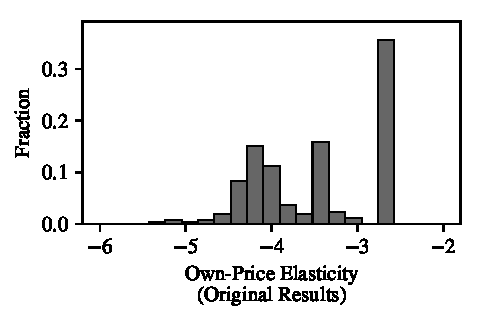
\includegraphics[width=0.32\textwidth]{includes/elasticity_histogram_1.pdf}
    \only<2->{
        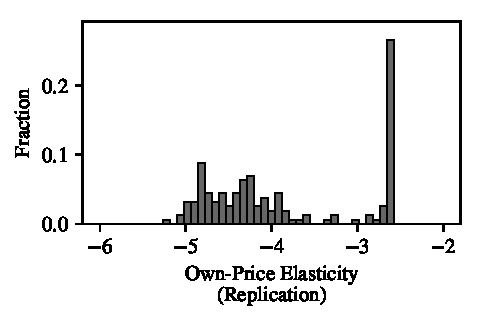
\includegraphics[width=0.32\textwidth]{includes/elasticity_histogram_2.pdf}
        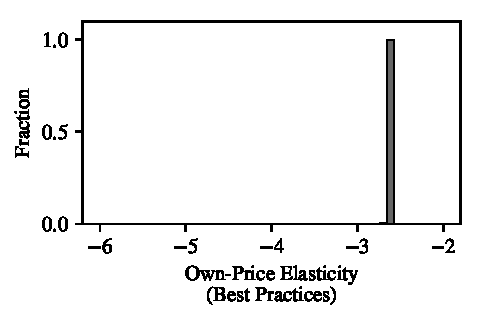
\includegraphics[width=0.32\textwidth]{includes/elasticity_histogram_3.pdf}
    }
    \begin{wideitemize}
        \item Variation in BLP estimates across different optimization algorithms and starting values has disillusioned some researchers \citep{knittel2014estimation}.
        \pause
        \item But there are some numerical best practices that you can follow to avoid these kinds of issues \citep{conlon2020best}.
        \begin{itemize}
            \item They're likely to be useful for most computation-heavy structural estimation, not just BLP!
        \end{itemize}
    \end{wideitemize}
\end{frame}

\begin{frame}{Nonlinear Optimization}
    \vspace{-\baselineskip}
    \begin{equation*}
        \hat{\theta} = \argmin_\theta Q(\theta)
    \end{equation*}
    \vspace{-0.5\baselineskip}
    \pause
    \begin{wideitemize}
        \item Set \alert{box constraints} $\theta \in [\underline{\theta}, \overline{\theta}]$ to preclude unrealistic and unstable guesses of $\theta$.
        \only<2>{
            \begin{itemize}
                \item E.g.\ huge $\Sigma$ values can make the inner loop unstable.
                \item Economic intuition and initial estimates will give a sense for reasonable bounds.
            \end{itemize}
        }
        \pause
        \item Check that 3-5 \alert{different starting values} $\theta \sim U(\underline{\theta}, \overline{\theta})$ give the same $\hat{\theta}$.
        \only<3>{
            \begin{itemize}
                \item For 2-step GMM, do this twice, once for each step (6-10 jobs total).
                \item If you have access to a cluster, each can be a separate job, run in parallel.
            \end{itemize}
        }
        \pause
        \item Prefer using \alert{gradient-based algorithms} for ``smooth'' problems like BLP.
        \only<4>{
            \begin{itemize}
                \item Avoid derivative-free methods like Nelder-Mead/simplex, which tend to work worse.
                \item I prefer trust-region algorithms, e.g.\ SciPy's \texttt{trust-constr} or Knitro if you have it.
            \end{itemize}
        }
        \pause
        \item Try to terminate on \alert{strict first-order conditions}, e.g.\ $\lVert\text{gradient}\rVert_\infty < $ \texttt{1e-8}.
        \only<5>{
            \begin{itemize}
                \item Inner loop should be tighter to prevent error ``bubbling up.'' PyBLP default is very tight.
                \item Can also check second-order conditions, i.e.\ Hessian eigenvalues are positive.
            \end{itemize}
        }
        \pause
        \item \alert{Configure your optimizer!} Defaults may not work for your setting.
    \end{wideitemize}
\end{frame}

\begin{frame}{Numerical Integration}
    \vspace{-\baselineskip}
    \begin{minipage}[c][4\baselineskip][c]{\textwidth}
        \begin{equation*}
            s_{jt} = \sum_{i \in \mathcal{I}_t} w_{it} \cdot \frac{\exp(\delta_{jt} + \mu_{ijt})}{1 + \sum_{k \in \mathcal{J}_t} \exp(\delta_{kt} + \mu_{ikt})} \only<2->{\approx \int \frac{\exp(\delta_{jt} + \mu_{ijt})}{1 + \sum_{k \in \mathcal{J}_t} \exp(\delta_{kt} + \mu_{ikt})} \,\mathrm{d}F(\mu_{it})}
        \end{equation*}
    \end{minipage}
    \vspace{-0.5\baselineskip}
    \pause
    \begin{wideitemize}
        \item Individual types $i$ are typically an \textit{approximation} to a population distribution.
        \pause
        \item Sometimes there are only a few types that we can integrate exactly.
        \only<3>{
            \begin{itemize}
                \item E.g.\ high- and low-income types $i \in \{1, 2\}$ with known shares $w_{1t}$ and $w_{2t} = 1 - w_{1t}$.
            \end{itemize}
        }
        \pause
        \item But usually we approximate the distribution with \alert{Monte Carlo} integration.
        \only<4>{
            \begin{itemize}
                \item Use a random number generator (RNG) to draw $|\mathcal{I}_t| \approx \text{1,000}$ of $(\nu_{it}, y_{it})$'s per market.
                \item Even better than your default RNG are \alert{quasi-Monte Carlo} sequences.
                \item I recommend scrambled Halton sequences. R: \cite{owen2017randomized}. Python: SciPy or PyBLP.
            \end{itemize}
        }
        \pause
        \item If you just need a few $\nu_{it} \sim N(0, I)$'s, try out \alert{Gauss-Hermite quadrature}.
        \only<5>{
            \begin{itemize}
                \item 10-100$\times$ fewer carefully-chosen $(w_{it}, \nu_{it})$'s that do just as well as Monte Carlo.
                \item Chosen to exactly integrate a polynomial expansion of the integrand.
            \end{itemize}
        }
        \pause
        \item \alert{Keep increasing $|\mathcal{I}_t|$} until your estimates stabilize across draws/starting values.
    \end{wideitemize}
\end{frame}

\begin{frame}{What Typically Goes Wrong}
    \begin{columns}
        \begin{column}{0.65\textwidth}
            \begin{wideitemize}
                \item<2-> Can see how $Q(\theta) = g(\theta)Wg(\theta)'$ varies with $\theta$.
                \item<3-> Here, there's a minimum but also some challenges.
                \begin{itemize}
                    \item<4-> \alert{Too few draws} $|\mathcal{I}_t|$ makes the objective ``choppy.''
                    \item<5-> \alert{Poorly-configured optimizers} can stop too early.
                \end{itemize}
                \item<6-> Different instruments give different objectives.
                \begin{itemize}
                    \item<7-> Even if they're all valid, some may be weaker.
                    \item<7-> Weaker means flatter and harder to optimize.
                \end{itemize}
            \end{wideitemize}
        \end{column}
        \begin{column}{0.35\textwidth}
            \vspace{0.5\baselineskip}
            \only<2->{\alt<2-5>{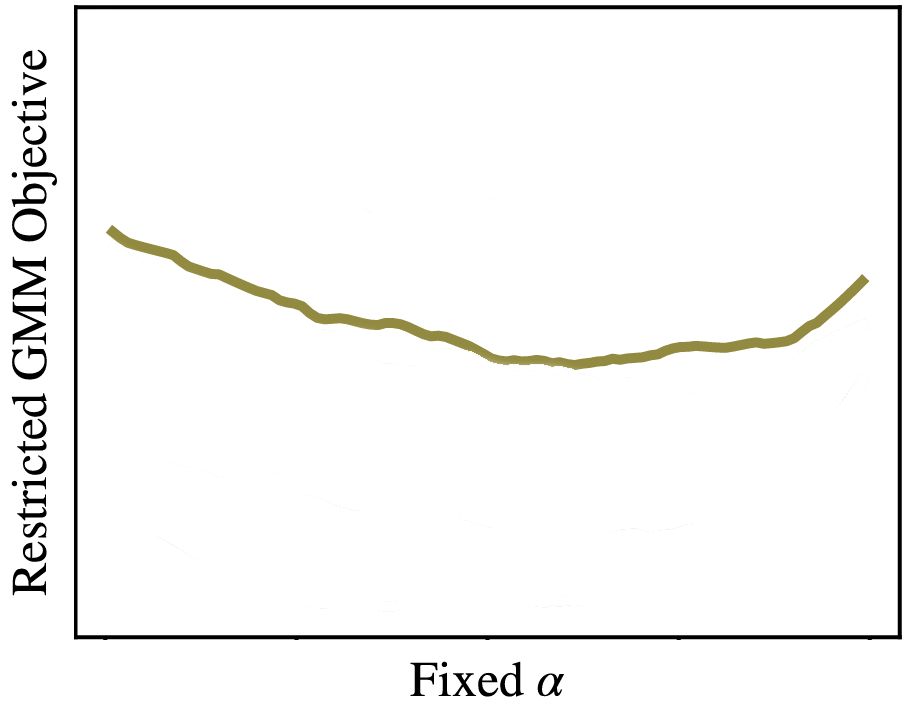
\includegraphics[width=\textwidth]{includes/profiled_objective_1.png}}{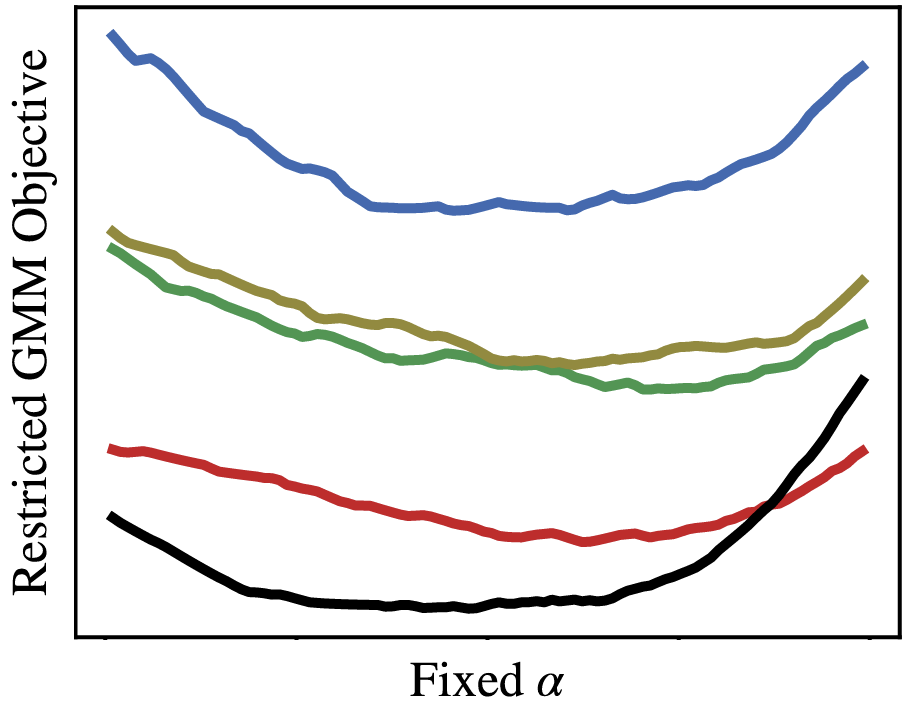
\includegraphics[width=\textwidth]{includes/profiled_objective_2.png}}}
        \end{column}
    \end{columns}
\end{frame}

\section{Differentiation Instruments}

\begin{frame}{Adding Instruments}
    \begin{wideitemize}
        \item For each new parameter in $(\Sigma, \Pi)$, we need another instrument in $z_{jt}$.
        \begin{itemize}
            \item If you have fewer moments than parameters, you're \textit{under-identified}.
        \end{itemize}
        \pause
        \item In general, I recommend starting with one instrument per parameter.
        \begin{itemize}
            \item Try to choose an instrument that ``targets'' that parameter.
            \item For example, a single strong cost-shifter that ``targets'' $\alpha$ on $p_{jt}$.
        \end{itemize}
        \pause
        \item This makes your estimation strategy clear, and makes optimization easier.
        \begin{itemize}
            \item \textit{Just-identified} models typically give $Q(\hat{\theta}) \approx 0$ at the optimum.
            \item This is regardless of your weighting matrix $W$, so you typically don't need 2-step GMM.
        \end{itemize}
        \pause
        \item Later, adding more can help with weakness and testing exclusion restrictions. 
    \end{wideitemize}
\end{frame}

\begin{frame}{Linear Regression Approximation}
    \begin{wideitemize}
        \item There's a lot of confusion about what instruments are needed for BLP estimation.
        \begin{itemize}
            \item Identification of nonlinear models like BLP can be challenging.
            \item See \cite{berry2014identification,berry2023nonparametric} for a more formal, nonparametric framework.
        \end{itemize}
        \pause
        \item Simplest case: 1 characteristic $x_{jt}$ (e.g.\ price), 1 demographic $y_{it}$ (e.g.\ income).
        \begin{equation*}
            u_{ijt} = (\beta + \sigma \nu_{it} + \pi y_{it}) x_{jt} + \xi_{jt} + \varepsilon_{ijt} 
        \end{equation*}
        \vspace{-1.5\baselineskip}
        \pause
        \item \cite{salanie2022fast} approximate the BLP model around $\sigma, \pi \approx 0$:
        \begin{equation*}
            \log\frac{s_{jt}}{s_{0t}} \approx \beta x_{jt} + \underbrace{\sigma^2 d_{jt}^x + \pi m_t^y x_{jt} + \pi^2 v_t^y d_{jt}^x}_{\text{Defined on the next slide.}} + \xi_{jt}
        \end{equation*}
        \vspace{-1.5\baselineskip}
        \pause
        \item Let's use our stronger intuition about linear regression to think about instruments!
    \end{wideitemize}
\end{frame}

\begin{frame}{Linear Regression Intuition}
    \vspace{-1\baselineskip}
    \begin{minipage}[c][4\baselineskip][c]{\textwidth}
        \begin{equation*}
            \log\frac{s_{jt}}{s_{0t}} \alt<3->{\approx}{=} \alert<2>{\beta x_{jt}} \only<3->{+ \alert<3-6>{\sigma^2 d_{jt}^x} \only<7->{+ \alert<7>{\pi m_t^y x_{jt}} + \alert<8>{\pi^2 v_t^y d_{jt}^x}}} + \xi_{jt} \only<3->{\quad\text{where}\quad d_{jt}^x = \Big(\frac{x_{jt}}{2} - \sum_{k \in \mathcal{J}_t} s_{kt} x_{kt}\Big) x_{jt}}
        \end{equation*}
    \end{minipage}
    \vspace{-0.5\baselineskip}
    \begin{wideitemize}
        \item If we set $\sigma = \pi = 0$ like on day 1, we get our familiar pure logit regression.
        \pause
        \only<2>{
            \begin{itemize}
                \item Use the same IV as before to target $\beta$: if $x_{jt} = p_{jt}$, a price IV; if exogenous, $x_{jt}$ itself.
            \end{itemize}
        }
        \pause
        \item To target $\sigma \neq 0$, need a measure of how ``differentiated'' $j$ is in terms of $x_{jt}$ within $t$.
        \only<3-6>{
            \begin{itemize}
                \item Can't use $d_{jt}^x$ itself because it depends on endogenous market shares $s_{kt}$.
                \pause
                \item Conventional choice was $\sum_{k \neq j} x_{kt}$, the\defcitealias{berry1995automobile}{BLP}\citetalias{berry1995automobile} instruments from day 1.
                \pause
                \item A stronger choice is $\sum_{k \neq j} (x_{jt} - x_{kt})^2$ or similar from \cite{gandhi2020measuring}.
                \pause
                \item We want \alert{cross-market choice set variation}, otherwise $d_{jt}^x$ is collinear with $x_{jt}^2$.
            \end{itemize}
        }
        \pause
        \item To target $\pi \neq 0$, we can interact $x_{jt}$ with mean within-market income $m_t^y$.
        \only<7-8>{
            \begin{itemize}
                \item We want \alert{cross-market demographic variation}, otherwise $m_t^y x_{jt}$ is collinear with $x_{jt}$.
                \item<8> Can technically identify $\pi$ from higher-order variation, e.g.\ in variance $v_t^y$.
            \end{itemize}
        }
        \only<9>{
            \item In your exercise, you'll target $(\beta, \sigma, \pi)$ with $z_{jt} = (x_{jt}, \sum_{k \neq j} (x_{jt} - x_{kt})^2, m_t^y x_{jt})$.
            \begin{itemize}
                \item If $x_{jt} = p_{jt}$, can replace $x_{jt}$ with fitted values $\hat{p}_{jt}$ from the price IV's first stage.
            \end{itemize}
        } 
    \end{wideitemize}
\end{frame}

\begin{frame}{Optimal Instruments}
    \begin{wideitemize}
        \item There are many valid instruments that satisfy exclusion restrictions $\E[\xi_{jt} \mid z_{jt}] = 0$.
        \begin{itemize}
            \item E.g.\ $z_{jt}$ itself, $z_{jt}^2$, $z_{jt}^3$, or any function $f(z_{jt})$ of $z_{jt}$.
        \end{itemize}
        \pause
        \item But adding a ton of instruments will bias your estimator.
        \begin{itemize}
            \item ``Many weak IVs'' problem is well-known for 2SLS \citep*{angrist1999jackknife}.
            \item Similar for nonlinear GMM \citep{han2006gmm,newey2009generalized}.
        \end{itemize}
        \pause
        \item \alert{Optimal IVs} overweight observations with $\xi_{jt}$ very sensitive to $\theta$ \citep{chamberlain1987asymptotic}:
        \begin{equation*}
            f^*(z_{jt}) = \E\bigg[\frac{\partial\xi_{jt}}{\partial\theta'} \Big| z_{jt}\bigg]
        \end{equation*}
        \vspace{-1.5\baselineskip}
        \pause
        \item Can be a bit tricky to compute, but with PyBLP it's just one line of code.
        \begin{itemize}
            \item In practice, can update your IVs along with your weighting matrix for a second GMM step.
        \end{itemize}
    \end{wideitemize}
\end{frame}

\section{Coding Exercise 2}

\begin{frame}{Coding Exercise 2}
    \begin{wideitemize}
        \item Try to do the second exercise before day 3's class, when I'll do it live.
        \begin{enumerate}
            \item Incorporating preference heterogeneity.
            \item Mixed logit estimation.
            \item Evaluating improvements to the price cut counterfactual.
        \end{enumerate}
        \pause
        \item Think critically about the limitations of the model you estimate.
        \begin{itemize}
            \item What dimensions of preference heterogeneity are missing?
        \end{itemize}
        \pause
        \item If you have time, try the supplemental exercises.
        \begin{itemize}
            \item Numerical integration alternatives.
            \item Optimal weights and instruments.
            \item Supply-side restrictions.
        \end{itemize}
    \end{wideitemize}
\end{frame}

\backupbegin

\begin{frame}[allowframebreaks,noframenumbering,plain]{References}
    \bibliography{includes/references.bib}
\end{frame}

\backupend

\end{document}